\ifx\mainfile\undefined
%  ========================================================================
%  Copyright (c) 2006-2011 The University of Washington
%
%  Licensed under the Apache License, Version 2.0 (the "License");
%  you may not use this file except in compliance with the License.
%  You may obtain a copy of the License at
%
%      http://www.apache.org/licenses/LICENSE-2.0
%
%  Unless required by applicable law or agreed to in writing, software
%  distributed under the License is distributed on an "AS IS" BASIS,
%  WITHOUT WARRANTIES OR CONDITIONS OF ANY KIND, either express or implied.
%  See the License for the specific language governing permissions and
%  limitations under the License.
%  ========================================================================
%
 
\documentclass [11pt, twoside] {uwthesis}

\usepackage{color}
\usepackage{url}
\usepackage{amsmath}
\usepackage{amsfonts}
\usepackage[bookmarks,
	hidelinks,
	plainpages=false,
	pdfpagelabels,
	pagebackref=true,
            ]{hyperref}
\renewcommand*{\backref}[1]{}% for backref < 1.33 necessary
\renewcommand*{\backrefalt}[4]{%
  \ifcase #1 %
    (No citations.)%
  \or
    (Cited on page #2.)%
  \else
    (Cited on pages #2.)%
  \fi
}

\newcommand{\biburl}[1]{{\tt<}\url{#1}{\tt>}}

\hypersetup{%
pdfauthor = {Daniel Chaim Halperin},
pdftitle = {Simplifying the Configuration of 802.11 Wireless Networks with Effective SNR},
pdfsubject = {Ph.D. Dissertation},
pdfkeywords = {},
pdfcreator = {University of Washington, Computer Science and Engineering},
pdfproducer = {},
bookmarksopen = {true},
pdfpagelayout = {TwoColumnRight},
}

\usepackage{footnotebackref}
%%%%%%%%%%%%%%%%%%%%%%%%%%%%%%%%%%%%%%%%%%%%%%%%%%%%%%
%%%        Formatting sections                     %%%
%%%%%%%%%%%%%%%%%%%%%%%%%%%%%%%%%%%%%%%%%%%%%%%%%%%%%%
\newcommand{\algref}[1]{Algorithm~\ref{#1}}
\newcommand{\chapref}[1]{Chapter~\ref{#1}}
\renewcommand{\eqref}[1]{Equation~\ref{#1}}
\newcommand{\figref}[1]{Figure~\ref{#1}}
\newcommand{\secref}[1]{\S\ref{#1}}
\newcommand{\tabref}[1]{Table~\ref{#1}}
\newcommand{\heading}[1]{\vspace{4pt}\noindent\textbf{#1}}
\newcommand{\topheading}[1]{\noindent\textbf{#1}}
\newcommand{\noheading}[0]{\vspace{4pt}\noindent}

%%%%%%%%%%%%%%%%%%%%%%%%%%%%%%%%%%%%%%%%%%%%%%%%%%%%%%
%%%        XXX and other warnings                  %%%
%%%%%%%%%%%%%%%%%%%%%%%%%%%%%%%%%%%%%%%%%%%%%%%%%%%%%%
\newcommand{\xxx}[1]{\textit{\color{red}XXX #1}}

%%%%%%%%%%%%%%%%%%%%%%%%%%%%%%%%%%%%%%%%%%%%%%%%%%%%%%
%%%        Units                                   %%%
%%%%%%%%%%%%%%%%%%%%%%%%%%%%%%%%%%%%%%%%%%%%%%%%%%%%%%
\usepackage{xspace}
\newcommand{\unitsep}{\texorpdfstring{\,}{ }}
\def\unit#1{% from: http://www.tex.ac.uk/cgi-bin/texfaq2html?label=csname "Defining a macro from an argument"
  \expandafter\def\csname #1\endcsname{\unitsep\text{#1}\xspace}%
}
\def\varunit#1#2{% from: http://www.tex.ac.uk/cgi-bin/texfaq2html?label=csname "Defining a macro from an argument"
  \expandafter\def\csname #1\endcsname{\unitsep\text{#2}\xspace}%
}
\unit{GHz}
\unit{MHz}
\unit{kHz}
\unit{Gbps}
\unit{Mbps}
\unit{KB}
\unit{dB}
\unit{dBi}
\unit{dBm}
\unit{W}
\unit{mW}
\varunit{uW}{$\mu$W}
\unit{ms}
\varunit{us}{$\mu$s}
\unit{h}
\unit{m}
\unit{s}
\unit{km}
\unit{cm}
\unit{mm}
\varunit{mmsq}{mm$^\text{2}$}
\varunit{insq}{in$^\text{2}$}
\newcommand{\degree}{\ensuremath{^\circ}\xspace}
\newcommand{\degrees}{\degree}
%%%%%%%%%%%%%%%%%%%%%%%%%%%%%%%%%%%%%%%%%%%%%%%%%%%%%%%%%%%%%%%%%%%%%%%%%%%%%%%%%%%%%%
% Euler for math | Palatino for rm | Helvetica for ss | Courier for tt
%
% From: http://www.tug.org/mactex/fonts/LaTeX_Preamble-Font_Choices.html
%%%%%%%%%%%%%%%%%%%%%%%%%%%%%%%%%%%%%%%%%%%%%%%%%%%%%%%%%%%%%%%%%%%%%%%%%%%%%%%%%%%%%%
\renewcommand{\rmdefault}{ppl} % rm
\usepackage[scaled]{helvet} % ss
\usepackage{courier} % tt
\usepackage{eulervm} % a better implementation of the euler package (not in gwTeX)
\normalfont
\usepackage[T1]{fontenc}
%%%%%%%%%%%%%%%%%%%%%%%%%%%%%%%%%%%%%%%%%%%%%%%%%%%%%%%%%%%%%%%%%%%%%%%%%%%%%%%%%%%%%%

%%%%%%%%%%%%%%%%%%%%%%%%%%%%%%%%%%%%%%%%%%%%%%%%%%%%%%
%%%        Figures                                 %%%
%%%%%%%%%%%%%%%%%%%%%%%%%%%%%%%%%%%%%%%%%%%%%%%%%%%%%%
\usepackage{graphicx}
% Caption package both lets you set the spacing between figure and caption
% and also makes the \figref{} point to the right place.
\usepackage[font=bf,aboveskip=6pt,belowskip=-4mm]{caption}
% Allow subfigures, make them bold
\usepackage[bf,BF,small]{subfigure}
% List of figures
\setcounter{lofdepth}{2}  % Print the chapter and sections to the lot

%%%%%%%%%%%%%%%%%%%%%%%%%%%%%%%%%%%%%%%%%%%%%%%%%%%%%%
%%%        Lists with reduced spacing              %%%
%%%%%%%%%%%%%%%%%%%%%%%%%%%%%%%%%%%%%%%%%%%%%%%%%%%%%%
\usepackage{enumitem}

%%%%%%%%%%%%%%%%%%%%%%%%%%%%%%%%%%%%%%%%%%%%%%%%%%%%%%
%%%        Fancy tables                            %%%
%%%%%%%%%%%%%%%%%%%%%%%%%%%%%%%%%%%%%%%%%%%%%%%%%%%%%%
\usepackage{tabulary}
\usepackage{booktabs}

%%%%%%%%%%%%%%%%%%%%%%%%%%%%%%%%%%%%%%%%%%%%%%%%%%%%%%
%%%        Formatting techniques/tools/etc.        %%%
%%%%%%%%%%%%%%%%%%%%%%%%%%%%%%%%%%%%%%%%%%%%%%%%%%%%%%
\newcommand{\term}[1]{\texttt{#1}}

\begin{document}
 
\textpages
\setcounter{chapter}{3} % Set to n-1!
\fi
%%%%%%%%%%%%%%%%%%%%%%%%%%%%%%%%%%

\cleardoublepage
\chapter{Effective SNR Model}
\label{chap:model}

As described in the previous chapter, the basic use of an Effective $E_b/N_0$ model for a faded multi-subchannel wireless link is to determine the average bit error rate of the link by aggregating across all subchannels. Conceptually, this is a simple process: simply determine the SNRs of the individual subcarriers, compute the individual BERs, average these BERs to calculate the Effective BER, and then determine the Effective SNR. However, each step of this operation is complex, because the model must be able to handle a wide range of transmitter and receiver techniques and their implementations. The challenge is to capture these complexities in a relatively simple model.

%%%%%%%%%%%%%%%%%%%%%%%%%%%%%%%%%%%%%%%%%%%%%%%%%%%%%%%%%%%%%%%%%%%%%%%%%%%%%%%%%%%%%%%%%%
\begin{figure}[ht]
\centering
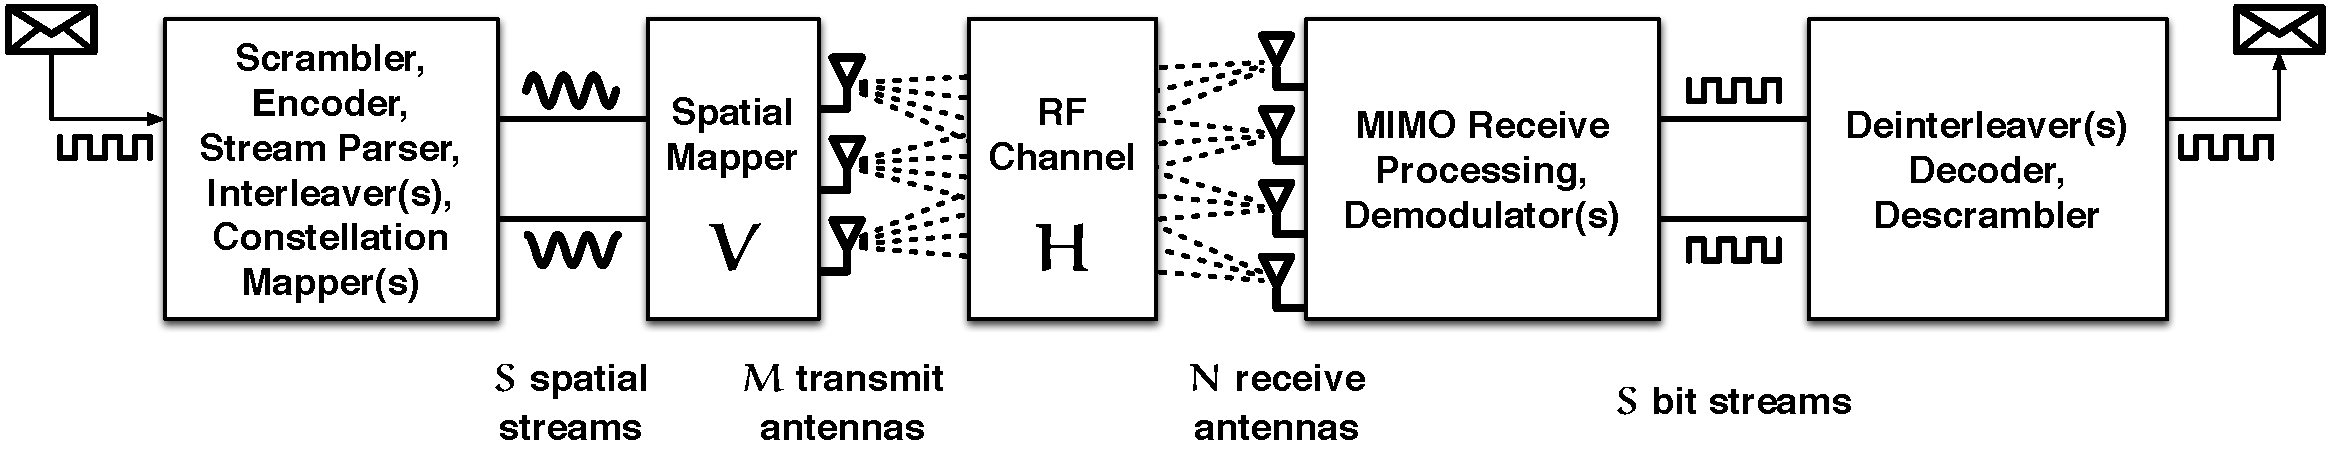
\includegraphics[width=\textwidth]{figures/11n_link_simplified_bigger_fonts.pdf}
\caption[An 802.11n link]{\label{fig:11n_link_simplified}A detailed view of a MIMO-OFDM link in the context of 802.11n.}
\end{figure}

\section{Overview of a MIMO-OFDM Link}
\figref{fig:11n_link_simplified} shows a detailed view of a MIMO-OFDM link in the context of 802.11n. The first block shows standard transmitter processing that generates $S$ spatial streams of modulated symbols from the packet. The internals of this block scramble the original packet to randomize the bits, add error correction, then split the coded bits across the $S$ spatial streams and interleave them between the OFDM subcarriers. These steps spread bits that are coded together across frequency- and spatially-diverse subchannels, after which the transmitter modulates the spread bits into the $S$ streams.

The second block is the \define{spatial mapper} $\mathbf{V}$, which maps the $S$ spatial streams to the $M$ transmit antennas. Different spatial mapping algorithms might map each stream to a single antenna, send a linear combination of each stream to each antenna, or (when $S<M$) use \define{Space-Time Block Codes (STBC)} to take advantage of the extra spatial diversity.

These signals then propagate across the RF channel $\mathbf{H}$ to the $N$ receive antennas. Note that although the figure shows a single RF channel $\mathbf{H}$, the channel can actually be different for every OFDM subcarrier. Consequently, transmitters with the ability to use beamforming can choose for each subcarrier $i$ a different spatial mapping $\mathbf{V}_i$ designed to make the best use of the channel $\mathbf{H}_i$.

After reception, the receiver employs one of many MIMO processing algorithms (i.e., MIMO equalizers) to disentangle the $S$ streams from the $N$ received signals, and demodulates the symbols to recover $S$ (potentially errored) streams of bits. This can be \define{hard demodulation} that simply outputs bits, or \define{soft demodulation} (\cite[\S5.3.1.3]{Sklar},\cite{Jamieson_PPR}) that includes a confidence value for each decoded bit based on the amount of noise in the channel.

In the last block, the receiver deinterleaves and decodes the coded bits, and then descrambles them to undo the transmit processing and recover the original bit stream. At this point, IEEE 802.11n devices typically compute the checksum of the received data and if correct, deliver the packet to the network stack on the host. This completes the description of the most important operations in the sending of a packet from transmitter to receiver in an 802.11n link.

I separated the link into the blocks shown to reflect the considerations that a practical model must handle. The transmitter operation in the first block is completely specified by the IEEE 802.11n standard and the selected rate and channel width. In contrast, the transmitter has a wide choice of spatial mapping matrices to implement unspecified antenna selection, transmit power control, and beamforming algorithms, among others. The receiver can adapt its configuration in response to the channel, for instance by disabling certain antennas and receive chains to save power. To process the received signals there are several MIMO equalizers, demodulation techniques, and error correction decoders that trade off complexity, cost, and performance, and the standard leaves these choices to the implementor. A practical model must be general and flexible to support these many algorithmic and implementation concerns.

%%%%%%%%%%%%%%%%%%%%%%%%%%%%%%%%%%%%%%%%%%%%%%%%%%%%%%%%%%%%%%%%%%%%%%%%%%%%%%%%%%%%%%%%%%
\begin{figure}[ht]
\centering
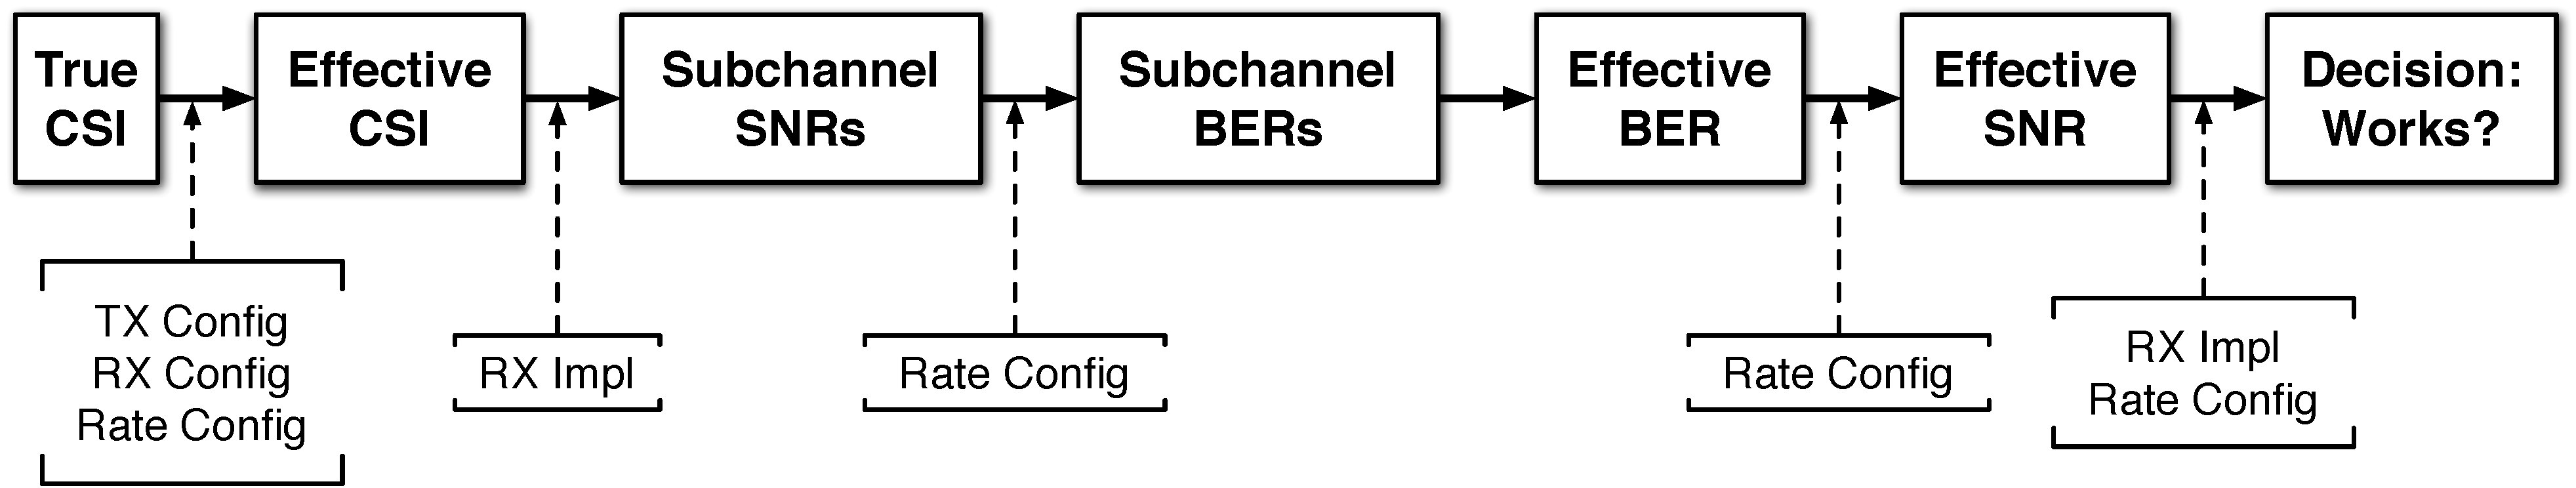
\includegraphics[width=\textwidth]{figures/esnr_model_overview.pdf}
\caption[Model overview]{\label{fig:model_overview}Overview of my Effective SNR-based model for wireless links. The model takes as input a CSI measurement (the ``true CSI'') along with a transmitter configuration, receiver configuration, rate configuration, and some information on the receiver implementation. The output is a single bit that determines whether the link will deliver a packet using the specified rate and device configurations.}
\end{figure}

\section{Model Overview}
\figref{fig:model_overview} gives an overview of my Effective SNR-based model for wireless links, designed to handle the cases described in the previous section. At the left, the primary input to the model is an RF measurement of the ground truth CSI for the wireless link. In the context of MIMO-OFDM technology such as IEEE 802.11n, this is the set of $N\times M$ matrices $\mathbf{H}_i$, where each matrix describes the MIMO channel between the $M$ transmit and $N$ receive antennas for one OFDM subcarrier.

The other inputs to the model are the configuration of the transmitter and receiver devices, the rate configuration, and some information about the receiver implementation. The final output of the model is a single bit that indicates whether the link will deliver a packet using the specified rate and device configurations. This model can flexibly handle a wide variety of applications: by varying the input transmitter, receiver, and rate configurations, we can solve all the problems described in \chapref{chap:problem}.

In the rest of this chapter, I explain each step of my model. To ease exposition, I start with the core Effective $E_b/N_0$ algorithm from Nanda and Rege~\cite{Nanda_EffectiveSNR}, by which I convert Subchannel SNRs to an Effective SNR, and use this Effective SNR to compute the output decision. I then make the model concrete in the context of IEEE 802.11n by explaining how we can calculate the Subchannel SNRs from the Effective CSI. Next I explain how to compute the Effective CSI, and thus support a variety of applications. Finally, I conclude by discussing how this model can be used in practical scenarios, including which side of the link performs the computation and what information is communicated.

\begin{table}
\centering
\begin{tabular}{cl}
\toprule%
Variable & Meaning\\
\midrule%
$M$ & Number of transmit antennas\\
$N$ & Number of receive antennas\\
$S$ & Number of spatial streams\\
$T$ & Number of OFDM subcarriers (tones) \\
$\mathbf{H}$ & Channel state matrix\\
$\mathbf{V}$ & Spatial mapping matrix\\
$C=ST$ & Number of subchannels \\
$i,j$ & Subchannel indices\\
$\rho$ & Signal-to-noise ratio (SNR) \\
$\beta$ & Bit error rate (BER) \\
$k$ & Number of bits per symbol \\
$\rho_\text{eff}, \beta_\text{eff}$ & Effective SNR or BER\\
$\mathbf{V}_i, \mathbf{H}_i$ & Per-subcarrier spatial mapping or channel state matrix\\
$m$ & Modulation and coding scheme (MCS) index \\
$\tau_m$ & Effective SNR threshold for MCS $m$ \\
\bottomrule
\end{tabular}
\caption{\label{tab:notation}Table of Notation}
\end{table}

%\begin{table}
%\centering
%\begin{tabular}{cc}
%\toprule%
%\textbf{Function} & \textbf{Computes}\\
%\midrule%
%$\text{BER}_k(\rho)$ & The bit error rate using the 802.11 modulation identified by $k$ at SNR $\rho$\\
%$Q(\cdot)$ & The tail probability (Complementary CDF) of the standard normal function. \\
%\bottomrule
%\end{tabular}
%\caption{\label{tab:functions}Table of functions}
%\end{table}

\begin{table}
\centering
%\footnotesize
\begin{tabular}{ccc}
\toprule
Modulation & Bits/Symbol ($k$) & BER$_k$($\rho$) \\
\midrule BPSK & 1 & $Q\left(\sqrt{2\rho}\right)$ \\
QPSK & 2 & $Q\left(\sqrt{\rho}\right)$\\
16-QAM & 4 & $\frac{3}{4}Q\left(\sqrt{\rho/5}\right)$\\
64-QAM & 6 & $\frac{7}{12}Q\left(\sqrt{\rho/21}\right)$\\
256-QAM$^*$ & 8 & $\frac{15}{32}Q\left(\sqrt{\rho/85}\right)$\\
\bottomrule
\end{tabular}
\caption[Bit error rate as a function of the symbol SNR for OFDM modulations]{\label{tab:ber_snr}Bit error rate as a function of the symbol SNR $\rho$ for narrowband signals and OFDM modulations. $Q$ is the standard normal CCDF. *IEEE 802.11ac will add 256-QAM.}
\end{table}

%%%%%%%%%%%%%%%%%%%%%%%%%%%%%%%%%%%%%%%%%%%%%%%%%%%%%%%%%%%%%%%%%%%%%%%%%%%%%%%%%%%%%%%%%%
\section{Computing Effective SNR from Subchannel SNRs}
At the core of my model is the Effective $E_b/N_0$ algorithm from Nanda and Rege~\cite{Nanda_EffectiveSNR}, which works as follows. Suppose that we are given a set of Subchannel SNRs, indexed such that $\rho_i$ corresponds to the SNR for the $i$th subchannel, $i\in1\dots C$.

The first step is to convert the Subchannel SNRs to Subchannel BERs. In \tabref{tab:ber_snr}, I give the formulas that relate SNR to BER for the modulations used in 802.11. These are adapted from textbook formulas~\cite[\S3.7.1 and \S7.9.3.1]{Sklar} to use the SNR that is measured by wireless NICs instead of the $E_b/N_0$ that is traditionally used in textbooks. Because different modulations have distinct constellations, each modulation has a slightly different error rate function identified as $\text{BER}_k$, where $k$ is the number of bits encoded by one symbol. I use $\text{BER}_k^{-1}$ to denote the inverse mapping from BER to SNR.

Because modern technologies use narrowband subchannels (such as OFDM subcarriers), we can assume that these formulas are accurate with respect to subchannel SNR and BER, unlike the packet-level SNR and BER for the entire link. Then we can compute the Effective BER (denoted $\beta_{\text{eff},k}$)
\begin{equation}
	\label{eq:effective_ber}
%	\tag{Effective BER}
	\beta_{\text{eff},k} = \frac{1}{C} \sum_{i}^{C} \text{BER}_k(\rho_i)
\end{equation}
and Effective SNR ($\rho_{\text{eff},k}$)
\begin{equation}
	\label{eq:effective_snr}
%	\tag{Effective SNR}
	\rho_{\text{eff},k} = \text{BER}_k^{-1}(\beta_{\text{eff},k}).
\end{equation}
%SoftRate estimates BER using internal receiver state~\cite{Vutukuru_SoftRate}. We compute it from channel measurements instead.

Note that the BER mapping and hence Effective SNR are functions of the modulation ($k$). That is, unlike the RSSI, a particular wireless channel will have four different Effective SNR values, one describing performance for each of the modulations. In practice, the interesting regions for the four Effective SNRs do not overlap because at a particular Effective SNR value only one modulation will be near the transition from useless (BER $\approx$0.5) to lossless (BER $\approx$0). When graphs in this paper are presented with an Effective SNR axis, we use all four values, each in the appropriate SNR range.

To compute the output decision bit that indicates whether the link will deliver packets, we simply compare the Effective SNR to an MCS-dependent threshold $\tau$:
\begin{equation}
\text{works?}_m = (\rho_{\text{eff},k} > \tau_m).
\end{equation}
Note that the MCS $m$ specifies the modulation and hence determines which $k$ to use. The thresholds $\tau_m$ are determined by the \emph{receiver implementation}, but are not link- or device-dependent. We can choose $\tau$ in a variety of ways, the most straightforward of which is via measurements over a wired link as in \figref{fig:snr_prr_attenuator}.

\subsection{Effective SNR Example}
\figref{fig:eff_example} presents an example of this core model for a SISO 802.11n link. The subchannels of this single-antenna link are simply the subcarriers, illustrated by the solid line. There is also one line for the packet SNR based on RSSI, and then four lines that each represent the Effective SNR for a different modulation. Note that the simpler modulations have lower Effective SNRs, but also perform much better at low rates. \tabref{tab:example_bers} shows the Effective BERs for this link.

\begin{figure}[t]
  \centering
  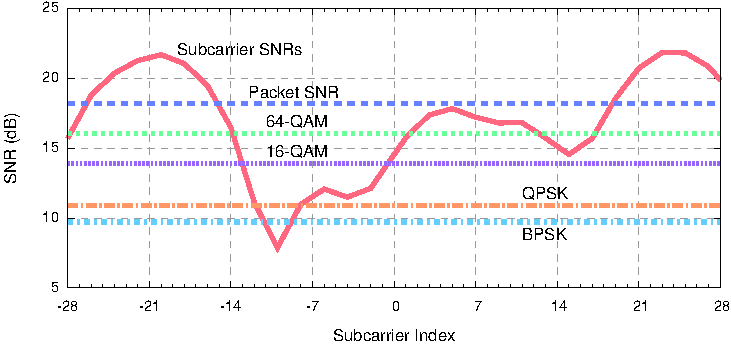
\includegraphics[width=0.9\textwidth]{figures/eff_snr_example.pdf}
  \caption[Packet SNR and Effective SNRs for a sample faded link]{Sample faded link showing the packet SNR and Effective SNRs for different modulations. BPSK has the lowest Effective SNR, but it needs less energy to decode.}
  \label{fig:eff_example}
\end{figure}

When the Effective SNRs are compared with the pre-determined thresholds for each rate, the model will correctly predict that the best working rate will be 39\Mbps. Note that these Effective SNRs are well below the packet SNR which is biased towards the stronger subcarriers (note the logarithmic $y$-axis scale). This link does a poor job of harnessing the received power because it is badly faded, so its SNR is a poor predictor of its rate.

\begin{table}[t]
	\centering
	\begin{tabular}{ccc}
	\toprule%
	Modulation & $\rho_\text{eff}$ (dB) & $\text{BER}_\text{eff}$\\
	\midrule%
	BPSK   &  9.7 & $8\times10^{-6}$\\
	QPSK   & 10.9 & $2\times10^{-4}$\\
	16-QAM & 13.9 & $1\%$\\
	64-QAM & 16.1 & $5\%$\\
	\bottomrule
	\end{tabular}
	\caption{\label{tab:example_bers}Effective SNRs and Effective BERs for the example link in \figref{fig:eff_example}.}
\end{table}

%%%%%%%%%%%%%%%%%%%%%%%%%%%%%%%%%%%%%%%%%%%%%%%%%%%%%%%%%%%%%%%%%%%%%%%%%%%%%%%%%
\section{Modeling the Receiver: Computing Subchannel SNRs from Effective CSI}
In the last section, I showed how the model of Nanda and Rege~\cite{Nanda_EffectiveSNR} can determine the Effective SNR from a list of Subchannel SNRs. In this section, I explain how to compute the Subchannel SNRs given the Effective Channel State Information of the link.

The \define{Effective CSI} is a $N\times S$ channel state matrix $\mathbf{H}'$, where each entry describes the gain and phase of each spatial stream as measured at each receive antenna. The first dimension of the Effective CSI is \emph{spatial streams}, not \emph{transmit antennas} as in the CSI matrix $\mathbf{H}$. From the point of view of receiver processing the number of transmit antennas used is not relevant, just how the transmitted streams are received after sender-side processing and propagation through the RF channel.

The IEEE 802.11 standards do not specify which algorithms the receiver uses to process received signals. However, my contact with Intel engineers and marketing documents from other chipset manufacturers indicate that a small set of techniques are likely chosen in practice.

\subsection{SISO links: $S=1,N=1$}
As in the example of \figref{fig:eff_example}, the SNR of a $1\times1$ channel matrix is simply the power of the single entry in the CSI matrix. There is one Subchannel SNR for each OFDM subcarrier:
\begin{equation}
	\rho_i = \left| \mathbf{H}'_i \right|^2.
\end{equation}

\subsection{SIMO links: $S=1,N>1$}
When there is a single stream and more than one receive antenna, there are two dominant algorithms used. The simpler technique is \define{antenna selection}, in which the antenna with the largest SNR is chosen, and then the SISO algorithm is used on that antenna's signal. The same antenna selection applies to all OFDM subcarriers.
\begin{equation}
	\rho_i = \left| \mathbf{H}'_{i,\hat{a}} \right|^2, \text{where antenna } \hat{a} \text{ has maximal Packet SNR}.
\end{equation}
Some older chipsets, such as the Intel PRO/Wireless 3945~\cite[\S3.5]{ipw3945} and Atheros AR5007~\cite{madwifi_diversity} used antenna selection by default.

The optimal SIMO technique is \define{maximal-ratio combining (MRC)}, which combines the multiple copies of the signal from the different receive antennas. The resulting subcarrier SNR is simply the sum of the SNRs of the individual entries:
\begin{equation}
	\label{eq:mrc}
	\rho_i = \sum_{a=1}^N \left| \mathbf{H}'_{i,a} \right|^2.
\end{equation}
MRC requires more hardware than antenna selection---one receive chain per antenna, instead of one receive chain total. But since spatial multiplexing techniques require multiple receive chains, 802.11n chipsets already have the hardware necessary to perform MRC. The additional computation is minimal, and the resulting gains are large, hence MRC is likely to be used for SIMO links by any 802.11n receiver. Production documentation for Atheros (e.g., the AR6004~\cite{ar6004}) and Realtek (e.g., the RTL8192SU~\cite{rtl8192su}) chipsets and the Intel 802.11n driver source code~\cite{iwlwifi} confirms this assertion.

Devices with more antennas than receive chains can use \define{hybrid selection-combining} algorithms. Such a device might first select the $n < N$ antennas that have the strongest Packet SNRs and then apply MRC to those.

\subsection{MIMO links: $S>1$}
When the transmitter uses spatial multiplexing, i.e.\ $S>1$, the receiver uses a MIMO equalizer to disentangle the streams from its $N\geq S$ receive antennas. For a MIMO link, there are a total of $C=TS$ values for Subchannel SNRs, one per subcarrier (tone) per stream. I denote these $\rho_{i,j}$ where $i$ is an index over tones and $j$ an index over streams. There are several possible techniques that do this; here I discuss the two algorithms most likely to be used in practice.

A \define{Minimum Mean Square Error (MMSE)} MIMO receiver is used by the Intel Wireless Wi-Fi Link 5300 and perhaps other 802.11n devices. For a single stream, MMSE is optimal and equivalent to MRC, and MMSE is near optimal for spatial multiplexing.

The SNR of the $j$th stream after MMSE processing for subcarrier $i$ is given by
\begin{equation}
\centering
\label{eq:mmse_snr}
\rho_{i,j} = \frac{1}{\mathbf{Y}_{jj}}-1, \text{ where }
\mathbf{Y} = \left((\mathbf{H}'_i)^\dagger \mathbf{H}'_i+I_S\right)^{-1}
\end{equation}
for $j \in [1,S]$ and $S\times S$ identity matrix $I_S$~\cite{Tse}. The operator $(\cdot)^\dagger$ indicates the \define{Hermitian}, or conjugate transpose of the input matrix.

The advantage of MMSE is that it performs well in most cases and has low computational cost, roughly the cost of matrix multiplication and inversion. An alternative is the \emph{Maximum Likelihood (ML)} decoder, but this has added complexity that scales with the size of the constellation, i.e., is exponential in the number of bits per symbol $k$. In the initial 802.11n chipsets, ML decoding was considered too complex to be practical, but this outlook has recently changed. Today, Intel's IWL6300 (successor to the IWL5300 mentioned above) uses ML decoding for the smaller constellations for which it is practical. Atheros uses a ``simplified maximum likelihood detector''~\cite{ar6004,Atheros_11nTechPaper} for all modulations that approximates ML performance but has lower complexity.

The task of estimating the per-stream SNR of the output from a maximum likelihood decoder is non-trivial. Existing estimation techniques, such as the approximation by Redlich et al.~\cite{Redlich_MLSNR}, have the same complexity as the full ML receiver, and are hence impractical for software implementation (though they may be suitable for use if implemented in hardware).

Instead, I observe that maximum likelihood decoding can be approximated as a $\approx$3\dB gain over MMSE for typical MIMO systems~\cite{Kumar_ml_mmse}. Thus, the practical solution I propose for my model is to always compute Effective SNR estimates using MMSE, and instead adapt the decision thresholds $\tau_m$ to reflect the use of ML decoding. This approximation is imprecise---the gains of ML will vary depending on the particular channel---but allows the model to flexibly handle many device implementations (even hybrid MMSE/ML such as in the IWL6300). The error is likely to be small for most channels.

\section{Applications: Adapting CSI to Compute Effective CSI}
By adapting the conversion between the CSI and the Effective CSI, my model supports a wide variety of application decisions. In this section I explain how to compute the Effective CSI $\mathbf{H}'$ from the CSI $\mathbf{H}$ for an illustrative set of these problems.

\heading{Antenna Selection.} There are $M$ rows and $N$ columns in the CSI that each correspond to one transmit or receive antenna. To implement antenna selection, we simply pick the subset of rows and columns that correspond to the desired antennas. Note that this includes both transmit antenna selection (e.g., when $S<M$, pick the best $S$ of the $M$ transmit antennas to send with) or receive antenna selection (e.g., when $N>S$, turn off the least useful of the excess antennas in order to reduce power consumption).

\heading{Channel Width Selection.} In 802.11n, a full 40\MHz CSI measurement would comprise 114 matrices $\mathbf{H}_i$. To implement channel width selection, we use only the $\mathbf{H}_i$ covered by the potential channel. For the lower 20\MHz channel, we would use the matrices corresponding to $i \in [1,56]$; for the upper 20\MHz channel we would use the matrices for $i \in [59,114]$. (Subcarriers 57 and 58 are not part of either 20\MHz channel because the 40\MHz channel does not need the same guard band.) This method can also predict performance using 5\MHz or 10\MHz channels as in 802.11j or SampleWidth~\cite{Chandra_SampleWidth}, and could support a potential future version of 802.11 that allows the devices to use non-contiguous tones as in SWIFT~\cite{Rahul_SWIFT}.

\heading{Transmit Power Control.} To emulate the effects of transmit power control, we can simply scale the entries in the matrices $\mathbf{H}_i$. When the transmitter reduces the transmit power uniformly across subcarriers, say by 3\dB, we multiple each matrix by the square root of the power change, in this example by $\sqrt{2}$. To model the effects of asymmetric power control across subchannels, e.g., water filling across streams or subcarriers, we can apply scaling differently to different parts of the channel matrix.

\heading{MCS (Rate) Selection.} For any of the above transmitter and receiver configurations, this process in conjunction with the core algorithms described in the last two sections can predict whether a particular MCS will reliably deliver packets. The CSI matrix may need to be slightly modified depending on the MCS, however. For instance, when using multiple streams the total amount of power is generally kept constant, so the Effective CSI must include a division of the transmit power across antennas. Similarly, some chipsets (e.g., IWL5300 and the Atheros-based Ubiquiti SR71-A~\cite{sr71a}) are unable to send at full power when using the highest modulations, because the peak-to-average power ratio (PAPR) is higher than the transmit amplifier(s) can support. For these chipsets, the Effective CSI must be scaled to compensate for the reduced transmit power when predicting the performance of the relevant modulations.

\heading{Spatial Mapping.} Spatial mapping algorithms determine how the different transmit streams are mapped to transmit antennas. These are implemented by the matrices $\mathbf{V}_i$, such that the Effective SNR is
\begin{equation}
	\mathbf{H}'_i = \mathbf{H}_i\mathbf{V}_i.
\end{equation}
I discuss the four types of spatial mapping techniques from the simplest to the most general.

\begin{itemize}
	\item In \define{direct mapping}, the transmitter maps each spatial stream directly to one of $S$ antennas; excess antennas go unused. After choosing the appropriate rows of $\mathbf{H}$ as described above under transmit antenna selection, the matrix $\mathbf{V}$ is the identity matrix $I_S$. We can combine transmit antenna selection and direct mapping using a $S \times M$ matrix $\mathbf{V}$ consisting of zeros except for the $S$ entries in different rows and columns that indicate which streams are mapped to which antennas. For $S=2$ and $M=3$, a direct mapping matrix using the first and third antennas would be
	\begin{equation*}
		\tag{Combined $2\times3$ TX Antenna Selection and Direct Mapping}
		\mathbf{V} = \begin{pmatrix}
		1 & 0 & 0\\
		0 & 0 & 1
		\end{pmatrix}.
	\end{equation*}

	\item In \define{indirect mapping}, the $S$ streams are mapped to $S$ antennas but in such a way as to be spread over multiple antennas. For instance, the IWL5300 uses the following indirect mapping for 3 streams and 20\MHz channels:
	\begin{equation*}
		\tag{IWL5300 $3\times3$}
		\mathbf{V} = \begin{pmatrix}
		e^{-i2\pi/16} & e^{-2i\pi/(80/33)} & e^{-2i\pi/(80/3)} \\
		e^{-i2\pi/(80/23)} & e^{-2i\pi/(48/13)} & e^{-2i\pi/(240/13)} \\
		e^{-i2\pi/(80/13)} & e^{-2i\pi/(240/37)} & e^{-2i\pi/(48/13)}
		\end{pmatrix}
	\end{equation*}
	Atheros uses Walsh (also called Hadamard) spreading. The $2\times2$ mapping is:
	\begin{equation*}
		\tag{Atheros $2\times2$}
		\mathbf{V} = \begin{pmatrix}
		1 & 1\\
		1 & -1
		\end{pmatrix}
	\end{equation*}
	
	\item When using \define{spatial expansion}, $S$ spatial streams are mapped to $M > S$ transmit antennas. Here, $\mathbf{V}$ is the product of an expansion matrix and one of the direct or indirect mapping matrices above. I show the case of $S=2$ and $M=3$ using a sample expansion matrix from the 802.11n standard:
	\begin{equation*}
		\tag{$3\times2$ Spatial Expansion}
		\mathbf{V} = \sqrt{\frac{2}{3}}\begin{pmatrix}
		1 & 0\\
		0 & 1\\
		1 & 0
		\end{pmatrix}\mathbf{V}',
	\end{equation*}
	where $\mathbf{V}'$ is a direct or indirect mapping matrix. The $\sqrt{2/3}$ factor above represents the even spreading of the power from 2 streams across 3 antennas.
	
	\item Finally, \define{beamforming} is a general technique for mapping streams to antennas. Beamforming can be thought of as a synthesis of indirect mapping, spatial expansion (if applicable) and transmit power control. The distinctive feature of beamforming compared with the above is that it is \emph{channel-aware}; in other words, the beamforming matrix is chosen to improve performance based on the known current channel $\mathbf{H}$. This means that beamforming can use different mapping matrices $\mathbf{V}_i$ for each subcarrier, unlike the prior techniques which are applied uniformly across tones. There are a large variety of techniques that use beamforming to improve the channel, but all can be represented in matrix form.
\end{itemize}

\heading{Higher-level Applications.} To implement applications that require the composition of multiple measurements, such as channel selection, path selection, or access point selection, we can repeat the steps above. For instance, two devices that wish to find the operating channel on which their link is fastest need only frequency-hop in unison and take CSI measurements for each frequency. They can then use the model to predict the achievable bitrate of each measured operating channel and select the fastest.

%%%%%%%%%%%%%%%%%%%%%%%%%%%%%%%%%%%%%%%%%%%%%%%%%%%%%%%%%%%%%%%%%%%%%%%%%%%%%%%%%%%%%%%%%%%%%%%%%%%%%%%%%
\section{Protocol Details}

\subsection{CSI Collection}
As with RSSI, receivers gather channel state information automatically while receiving a packet; the OFDM and MIMO equalizers described above fundamentally rely on CSI to decode the received signal. This \emph{passive collection} of CSI via overheard transmissions suffices for most applications, such as rate selection. When a more comprehensive CSI measurement is needed, the transmitter can send a sounding packet~\cite[\S20.3.13.1]{80211n} at a wider bandwidth or using more streams probe the extra dimensions. For the special case of additional spatial streams, 802.11n includes a mechanism to send a modified packet with \define{extension spatial streams}~\cite[\S20.3.9.4.6]{80211n} such that the receiver can measure the full channel during the preamble but that does not change the rate or number of streams used for the data portion.

\subsection{Transmitter or Receiver Calculations}
Effective SNR calculations can be performed by either side of the link, and each has advantages. The primary tradeoff is between the amount of data shared (the party performing the calculation needs up-to-date CSI) and hardware complexity.

\heading{Necessary Information.} To make the calculations and choose an operating point, the following three pieces of information are needed:
\begin{itemize}
	\item Up-to-date CSI measurements including all relevant subchannels.
	\item Receiver's MCS-specific Effective SNR thresholds.
	\item Transmitter's capabilities including possible spatial mapping matrices, as well as any implementation-specific oddities (such as Intel's reduction of transmit power by up to 5\dB for the highest 64-QAM single-stream encodings).
\end{itemize}

\heading{Transmitter-side Computation.} The receiver's MCS thresholds are fixed for a particular model of NIC; they can be shared by the receiver once, e.g., during association. The transmitter also needs up-to-date CSI, either obtained via feedback or estimated implicitly from the reverse path. When the receiver feeds CSI back to the transmitter, this process adds latency and reduces airtime efficiency. 802.11n includes mechanisms to limit these effects via rapid feedback protocols~\cite[\S9.19.2]{80211n} and compressed CSI feedback formats~\cite[\S20.3.12.2.5]{80211n}.

Alternatively, the transmitter can estimate the CSI implicitly when receiving packets, such as ACKs, sent by the receiver. This in turn mandates that the receiver inform the transmitter of its spatial mapping matrices, and use all its antennas to send these packets. Note that some receivers, such as the Intel IWL5100, have more receive antennas than transmit chains. Some of those devices cannot send on all antennas, and implicit feedback would not work; the other receivers would need to alternate transmit antennas while the transmitter used CSI Sampling and Fusion~\cite{Crepaldi_CSI_SF} to build up a complete CSI. The use of implicit feedback also requires devices to use the the 802.11n calibration process to compensate for hardware differences in the measured transmit and receive chains and those that will be used when the two devices swap roles.

\heading{Receiver-side Computation.} The other approach is for the receiver to perform the computations and make the application decisions. To do this, the receiver can use the new 802.11n Link Adaptation Control field~\cite[\S7.1.3.5a]{80211n} that can embed feedback in packet headers, including ACKs, to directly request a particular MCS, select antennas, or request a particular beamforming (or other spatial mapping) matrix.

This obviates sending CSI and speeds up the protocols, but instead requires that the receiver understand the full extent of the transmitter's capabilities. The transmitter and receiver share some of these details, such as number of transmit antennas and whether a device supports optional 802.11n features, on association. But the standard does not include a method by which a transmitter can share its spatial mapping matrices, and it's not immediately clear that this would sufficiently capture all implementations. The other drawback is that it complicates receiver hardware; many 802.11 manufacturers have targeted systems with asymmetric capabilities such that the access point shoulders all the computation load, reducing the complexity and hence cost of the client which need only support basic feedback.

%%%%%%%%%%%%%%%%%%%%%%%%%%%%%%%%%%%%%%%%%%%%%%%%%%%%%%%%%%%%%%%%%%%%%%%%%%%%%%%%%%%%%%%%%%%%%%%%%%%%%%%%%
\section{Comparison to Other Techniques}
\tabref{tab:algorithm_comparison} includes a comparison of my Effective SNR model to other techniques that use physical layer or other low-level information to predict the performance of a wireless link. As I presented in the previous section, RSSI is available in today's devices, but does not accurately predict performance for 802.11a/g due to its inability to capture frequency-selective fading; the use of MIMO in 802.11n only exacerbates this deficiency.

\begin{table}
\begin{tabular}{ccccccc}
\toprule
\multirow{2}{*}{Algorithm} & \multirow{2}{*}{802.11a/b/g} & 802.11n & Antenna & \multirow{2}{*}{TX Power} & Channel & \multirow{2}{*}{Real NICs} \\
& & (MIMO) & Selection & & Width \\
\midrule
RSSI & ? & & & & & \checkmark\\
SoftRate~\cite{Vutukuru_SoftRate} & \checkmark \\
AccuRate~\cite{Sen_AccuRate} & \checkmark & & & \checkmark & \checkmark \\
EEC~\cite{Chen_EEC} & \checkmark & & & & & \checkmark \\
Effective SNR & \checkmark & \checkmark & \checkmark & \checkmark & \checkmark & \checkmark\\
\bottomrule
\end{tabular}
\caption[Comparison of link error rate prediction algorithms]{\label{tab:algorithm_comparison}A comparison of Effective SNR to other recent algorithms that purport to predict the performance of a wireless link. Effective SNR can predict packet delivery in the largest space because it looks at the raw channel response, whereas the other techniques mostly apply only to single-stream links with fixed antennas and transmit power.}
\end{table}

SoftRate~\cite{Vutukuru_SoftRate} and EEC~\cite{Chen_EEC} both use information from the error correction hardware to accurately measure the Effective BER of the \emph{current} configuration and work well for rate selection using adjacent 802.11a/b/g rates, but cannot predict the performance using other configurations.

AccuRate~\cite{Sen_AccuRate} uses the measured receive error vectors as input to a full channel simulator; like my model this procedure can estimate the Effective BER of all modulations in the current configuration. However, these computations are computationally expensive and do not work across other applications. The exception is transmit power control; I believe this can be simulated by scaling the error vectors although this approach was not explored by the authors.

In contrast, Effective SNR extends to a significantly larger class of applications than the other techniques because its computations are aware of the low-level physical-layer effects of the RF channel, including frequency- and spatially-selective fading. My model is broadly compatible with 802.11n and requires no hardware changes. As part of my thesis I built a prototype implementation using a commercial Intel NIC. In the rest of this thesis, I present my prototype implementation of Effective SNR and demonstrate that it works well and supports a wide space of applications.

\begin{comment}
\color{red}
\section{Omitted text}
Coding interacts with the notion of Effective SNR in a way that is difficult to analyze. One challenge is that the ability to correct bit errors depends on the position of the errors in the data stream. To sidestep this problem, we rely on the interleaving that randomizes the coded bits across subcarriers and spatial streams. Assuming perfect interleaving and robust coding, bit errors in the stream should look no different from bit errors for flat channels (but at a lower SNR). Thus our estimate of the effective BER in \eqref{eq:effective_ber} will accurately reflect the uncoded error performance of the link. Our algorithm now proceeds as in the case of a flat-fading channel described above: we take the computed Effective SNR value and use the measurements from a flat-fading link (\figref{fig:snr_prr_attenuator}) to determine transmission success or failure. As in CHARM~\cite{Judd_CHARM}, we support different packet lengths with different SNR thresholds.

Note that this procedure differs from the typical approach of simulation-based analyses~\cite{Kant_fla, Liu_EESM, Nortel_3g}, that instead map the \emph{uncoded} BER estimate such as we compute to a \emph{coded} BER estimate by means of a simple log-linear approximation. They then use the coded BER estimate, and the length of the target transmission, to directly compute the packet delivery rate of the link. We believe our method of thresholding the Effective SNR is better because it directly accommodates variation in the receiver implementation. Different devices may have different \emph{noise figures}, a measure of how much signal strength is lost in the internal RF circuitry of the NIC\@. They may implement soft Viterbi decoders with more or fewer soft bits for their internal state, or indeed might do hard decoding instead. A receiver could use the optimal Maximum Likelihood MIMO decoder that has exponential complexity for small constellations like BPSK, but revert to the imperfect but more efficient MMSE at higher modulations. All of these can be easily expressed, albeit maybe approximately, as (perhaps modulation-dependent) shifts in the Effective SNR thresholds. In contrast, changing these parameters in the simulation approach involves changing the internals of the calculation.

\color{black}
\end{comment}

%\heading{802.11 Packet Reception.}
%The model must account for the action of the 802.11 receiver on the received signal. This is a complex process described in many pages of the 802.11n specification~\cite{80211n}. Our challenge is to capture it well enough with a fairly simple model. We begin by describing the main steps involved (\figref{fig:ofdm_decoding}).
%
%First, MIMO processing separates the signals of multiple spatial streams that have been mixed by the channel. As wireless channels are frequency-selective, this operation happens separately for each subcarrier. The demodulator converts each subcarrier's symbols into the bits of each stream from constellations of several different modulations (BPSK, QPSK, 16-QAM, 64-QAM). This happens in much the same way as demodulating a narrowband channel. The bits are then deinterleaved to undo an encoding that spreads errors that are bursty in frequency across the data stream. A parallel to serial converter combines the bits into a single stream. Forward error correction at any of several rates (1/2, 2/3, 3/4, and 5/6) is then decoded. Finally, the descrambler exclusive-ORs the bitstream with a pseudorandom bitmask added at the transmitter to avoid data-dependent deterministic errors.
%
%\begin{figure*}[ht!]
%\centering
%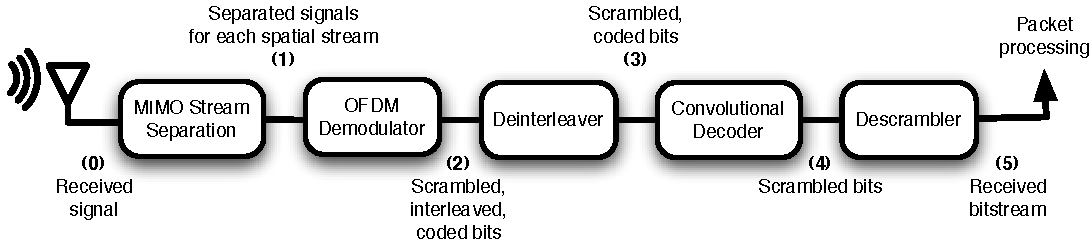
\includegraphics[width=6in]{figures/esnr/mimo_ofdm_decoding_process.pdf}
%\caption[The 802.11n MIMO-OFDM decoding process]{\label{fig:ofdm_decoding} The 802.11n MIMO-OFDM decoding process. MIMO receiver separates the RF signal~(0) for each spatial stream~(1). Demodulation converts the separated signals into bits~(2). Bits from the multiple streams are deinterleaved and combined~(3) followed by convolutional decoding~(4) to correct errors. Finally, scrambling that randomizes bit patterns is removed and the packet is processed~(5).}
%\end{figure*}
%
%\heading{Modeling Delivery.}
%We build our model up from narrowband demodulation. 
%Standard formulas summarized in \tabref{tab:ber_snr} relate SNR (denoted $\rho$) to bit-error rate (BER) for the modulations used in 802.11~\cite{Goldsmith}. CSI gives us the SNR values ($\rho_s$) to use for each subcarrier. For a SISO system, $\rho_s$ is given by the single entry in $H_s$.
%
%In OFDM, decoding is applied across the demodulated bits of subcarriers. If we assume frequency-flat fading for the moment, then all the subcarriers have the same SNR\@. The link will behave the same as in our wired experiments in which RSSI reflect real performance and it will be easy to make predictions for a given SNR and modulation combination. We can use \figref{fig:snr_prr_attenuator} to measure the fixed transition points between rates and thus make our choice.
%
%Frequency-selective fading complicates this picture as some weak subcarriers will be much more likely to have errors than others that are stronger. To model a link in this case, we turn to the notion of an \textbf{\em Effective SNR}\@. This is defined as the SNR that would give the \emph{same error performance on a narrowband channel}~\cite{Nanda_EffectiveSNR}. For example, the links in \figref{fig:example_fsf_shape} will have Effective SNR values that are nearly equal because they perform similarly, even though their RSSIs are spread over 15\dB.
%
%The Effective SNR is \emph{not} simply the average subcarrier SNR; indeed, assuming a uniform noise floor, that average is indeed equivalent to the packet SNR derived from the RSSI\@. Instead, the Effective SNR is biased towards the weaker subcarrier SNRs because it is these subcarriers that produce most of the errors. If we ignore coding for the moment, then we can compute the Effective SNR by averaging the subcarrier BERs and then finding the corresponding SNR\@. That is:
%\begin{equation}
%\label{eq:effective_ber}
%	\beta_{\text{eff},k} = \frac{1}{52} \sum \text{BER}_k(\rho_s)
%\end{equation}
%\begin{equation}
%\label{eq:effective_snr}
%	\rho_{\text{eff},k} = \text{BER}_k^{-1}(\beta_{\text{eff},k})
%\end{equation}
%We use $\text{BER}_k^{-1}$ to denote the inverse mapping, from BER to SNR\@. We have also called the average BER across subcarriers the effective BER, $\beta_{\text{eff}}$. SoftRate estimates BER using internal receiver state~\cite{Vutukuru_SoftRate}. We compute it from channel measurements instead.





%%%%%%%%%%%%%%%%%%%%%%%%%%%%%%%%%%
\ifx\mainfile\undefined
%
% ==========   Bibliography   ==========
%
%\nocite{*}   % include everything in the uwthesis.bib file
\bibliographystyle{plain}
\bibliography{dhalperi_thesis}

\end{document}
\fi
